%% Overleaf			
%% Software Manual and Technical Document Template	
%% 									
%% This provides an example of a software manual created in Overleaf.

\documentclass{../ol-softwaremanual}

% Packages used in this example
\usepackage{graphicx}  % for including images
\usepackage{microtype} % for typographical enhancements
\usepackage{minted}    % for code listings
\usepackage{amsmath}   % for equations and mathematics
\setminted{style=friendly,fontsize=\small}
\renewcommand{\listoflistingscaption}{List of Code Listings}
\usepackage{hyperref}  % for hyperlinks
\usepackage[a4paper,top=4.2cm,bottom=4.2cm,left=3.5cm,right=3.5cm]{geometry} % for setting page size and margins

\usepackage[english, greek]{babel}

\usepackage{subfig}

\usepackage{incgraph,tikz}

\usepackage{filemod}





\usepackage{rotating}


% Custom macros used in this example document
\newcommand{\doclink}[2]{\href{#1}{#2}\footnote{\url{#1}}}
\newcommand{\cs}[1]{\texttt{\textbackslash #1}}

\begin{document}
	
	
	\begin{titlepage}
		
		
		% Frontmatter data; appears on title page
		\title{\en Robustness Diagrams \\}
		\version{0.3}
		\softwarelogo{
\includegraphics[scale=0.4]{../CarBazaar_logo.png}}		
		
	\end{titlepage}
	
	
	\maketitle
	
	\newpage
	
	\center{\textbf{Μέλη Ομάδας}}
	
	\vspace{20pt}
	
	
	
	\begin{table}[htbp!]
		
		\begin{tabular}{llll}
			Μεμελετζόγλου Χαρίλαος & 1069364 & \en st1069364@ceid.upatras.gr & 4o Έτος   \\ 
			\\ Λέκκας Γεώργιος      &      1067430    &   \en st1067430@ceid.upatras.gr & 4o Έτος  \\
			\\ Γιαννουλάκης Ανδρέας        &   1067387       & \en st1067387@ceid.upatras.gr & 4o Έτος           \\
			\\ Κανελλόπουλος Ιωακείμ        &  1070914        &    \en st1070914@ceid.upatras.gr & 4o Έτος        \\ 
		\end{tabular}
	\end{table}
	
	\center{\textbf{Υπεύθυνοι Παρόντος Τεχνικού Κειμένου}}
	
	\vspace{20pt}
	
	\begin{table}[htbp!]
		\begin{tabular}{ll}
			Μεμελετζόγλου Χαρίλαος & \en Editor \\
			\\ Λέκκας Γεώργιος      &   \en  Editor \\
			\\ Γιαννουλάκης Ανδρέας & \en Contributor \\
			\\ Κανελλόπουλος Ιωακείμ & \en Contributor \\ 
		\end{tabular}
	\end{table}
	
	\center{\textbf{Αλλαγές στην έκδοση \en v0.3 \gr}}
	
	\flushleft
	
	Αφαίρεση της λανθασμένης ακμής μεταξύ του \en Boundary object "\gr Οθόνη Καταχώρησης Αγγελίας Οχήματος\en"\gr και του Ελεγκτή \en"\gr Υπαρκτό Όχημα\en?"\gr, στο \en robustness diagram \gr του \en use case \en"\gr Ανάρτηση Αγγελίας Πώλησης Οχήματος\en"\gr
	
	
	\newpage
	
	\center{\textbf{Εργαλεία που χρησιμοποιήθηκαν}}
	
	\vspace{20pt}
	\flushleft
	Χρησιμοποιήθηκε το \en \doclink{https://www.overleaf.com/}{Overleaf} \gr και το \en \doclink{https://www.texstudio.org/}{TexStudio} \gr για την συγγραφή του \LaTeX\ κώδικα. \break
	
	Για την δημιουργία του λογότυπου, χρησιμοποιήθηκε το εργαλείο \en \doclink{https://www.adobe.com/express/create/logo}{Adobe Express} . \gr \break
	
	Για την δημιουργία των \en Robustness Diagrams \gr χρησιμοποιήθηκε το \en \doclink{https://www.visual-paradigm.com/}{Visual Paradigm} . \gr \break 
	
	\newpage
	
	\center{\textbf{\en Robustness Diagrams \gr}}
	\flushleft
	
	Οι εναλλακτικές ροές του κάθε \en Use Case \gr φαίνονται στο αντίστοιχο \en Robustness Diagram \gr, με κόκκινες ακμές και αντικείμενα. \break
	
	Για την ευκολότερη αντιστοίχιση ενός \en Use Case \gr στο αντίστοιχο \en Robustness Diagram \gr, παραθέτουμε και το κείμενο της κάθε Περίπτωσης Χρήσης, πριν το διάγραμμα που προκύπτει. \break
	
	Ακολουθεί αντιστοίχηση των Οντοτήτων των διαγραμμάτων, στις αντίστοιχες κλάσεις του \en Domain Model \gr.
	
	\begin{itemize}
		\item Οντότητα \textit{Αγγελία} : Αντιστοιχεί στην (γενική) κλάση \en \textbf{Listing}\gr
		\item Οντότητα \textit{Αγγελία Οχήματος} : Αντιστοιχεί στην κλάση \en \textbf{CarListing}\gr
		\item Οντότητα \textit{Αγγελία Ανταλλακτικού} : Αντιστοιχεί στην κλάση \en \textbf{SparePartListing}\gr
		\item Οντότητα \textit{Μηνιαία Δόση} : Αντιστοιχεί στην κλάση \en\textbf{MonthlyInstallment}\gr
		\item Οντότητα \textit{Συναλλαγή} : Αντιστοιχεί στην κλάση \en \textbf{Transaction}\gr
		\item Οντότητα \en \textit{TransactionLog} \gr : Αντιστοιχεί στην κλάση \en \textbf{TransactionLog}\gr
		\item Οντότητα \textit{Απόδειξη} : Αντιστοιχεί στην κλάση \en \textbf{Invoice}\gr
		\item Οντότητα \textit{'Ελεγχος Οχήματος} : Αντιστοιχεί στην κλάση \en \textbf{CarInspection}\gr
		\item Οντότητα \textit{Ελεγκτής} : Αντιστοιχεί στην κλάση \en \textbf{Inspector}\gr
		\item Οντότητα \textit{Τοποθεσία} : Αντιστοιχεί στην κλάση \en \textbf{Location}\gr
		\item Οντότητα \textit{Ανταλλακτικό} : Αντιστοιχεί στην κλάση \en \textbf{SparePart}\gr
		\item Οντότητα \textit{Φωτογραφία} : Αντιστοιχεί στην κλάση \en \textbf{Photograph}\gr
		\item Οντότητα \textit{Αναφορά Αγγελίας} : Αντιστοιχεί στην κλάση \en \textbf{ListingReport}\gr
		\item Οντότητα \textit{Διαφήμιση} : Αντιστοιχεί στην κλάση \en \textbf{Advertisment}\gr
		\item Οντότητα \textit{Ανταλλαγή Οχήματος} : Αντιστοιχεί στην κλάση \en \textbf{CarExchange}\gr
		\item Οντότητα \textit{Σύγκριση Οχημάτων} : Αντιστοιχεί στην κλάση \en \textbf{CarCompare}\gr
		\item Οντότητα \textit{Μεταφορά Οχήματος} : Αντιστοιχεί στην κλάση \en \textbf{CarTransportation}\gr
		\item Οντότητα \textit{Μεταφορέας} : Αντιστοιχεί στην κλάση \en \textbf{Transporter}\gr
		\item Οντότητα \en \textit{Test Drive} \gr : Αντιστοιχεί στην κλάση \en \textbf{TestDrive}\gr
		\item Οντότητα \textit{Κατάστημα Αντιπροσωπείας} : Αντιστοιχεί στην κλάση \en \textbf{DealershipStore}\gr
		\item Οντότητα \textit{Αναζήτηση Οχήματος} : Αντιστοιχεί στην κλάση \en \textbf{CarSearch} \gr
		\item Οντότητα \en \textit{CarListingsStatisticsLog} \gr : Αντιστοιχεί στην κλάση \en \textbf{CarListingsStatisticsLog} \gr		
	\end{itemize}
	
	Στα διαγράμματα εμφανίζονται οι Οντότητες \textit{Αποτελέσματα Αναζήτησης} και \textit{Αποτελέσματα Σύγκρισης}, που αντιστοιχούν στα εφήμερα αντικείμενα των αντίστοιχων \en  Use Cases \gr. \\
	
	Επίσης, η Οντότητα \textit{Κωδικός Ασφαλείας}, αντιστοιχεί στο εφήμερο αντικείμενο του κωδικού ασφαλείας, που αποστέλλεται στο \en email \gr του χρήστη, κατά την έναρξη της αγοράς οχήματος.
	
	
	\newpage
	
	\paragraph{\en Use Case 1: \gr Ανάρτηση Αγγελίας Πώλησης Οχήματος}
	\centering
	
	\begin{enumerate}
		
		\item Ο χρήστης επιλέγει \en"\gr Ανάρτηση Αγγελίας Οχήματος\en" \gr στο αρχικό μενού
		\item Το σύστημα εμφανίζει την οθόνη Καταχώρησης Αγγελίας Πώλησης Οχήματος
		\item Ο χρήστης εισάγει την τοποθεσία του, τον τίτλο της αγγελίας, στοιχεία του οχήματος όπως μάρκα, μοντέλο, έτος κυκλοφορίας, χιλιόμετρα, κυβικά, τύπος καυσίμου, χρώμα, αριθμός πινακίδας, κλπ
		\item Το σύστημα εντοπίζει τον χρήστη, ελέγχει πως όντως κυκλοφορεί αντίστοιχο μοντέλο αυτοκινήτου στην αγορά και δημιουργεί την οντότητα \en \textit{Car} \gr, όπου αποθηκεύονται προσωρινά τα στοιχεία του οχήματος. Έπειτα, εμφανίζει την Οθόνη Ανάρτησης Εγγράφων Πιστοποίησης Κατάστασης Οχήματος
		\item Ο χρήστης ανεβάζει τα απαραίτητα έγγραφα που έχουν προκύψει από τον έλεγχο του οχήματος		
		\item Το σύστημα υπολογίζει μια εκτίμηση της τιμής του οχήματος, με βάση την κατάστασή του και εμφανίζει την Οθόνη Τιμής Οχήματος
		\item Ο χρήστης επιλέγει να συνεχίσει με την προτεινόμενη τιμή ή εισάγει δικιά του
		\item Το σύστημα ελέγχει αν ο χρήστης αποδέχθηκε την προτεινόμενη τιμή. Σε περίπτωση μη-αποδοχής, ελέγχει αν η τιμή που εισήγαγε ο χρήστης παρουσιάζει μεγάλη απόκλιση από την προτεινόμενη τιμή		
		\item Το σύστημα μεταφέρει τον χρήστη στην οθόνη Εισαγωγής Φωτογραφιών και Περιγραφής Οχήματος
		\item Ο χρήστης προσθέτει το κείμενο της περιγραφής και αναρτά τις φωτογραφίες του αυτοκινήτου
		\item Το σύστημα αφού ελέγξει πως συμπληρώθηκαν τα πεδία περιγραφής και φωτογραφιών, δημιουργεί την αγγελία (Οντότητα \en \textit{CarListing}\gr)
		\item Το σύστημα ανακτά τα στοιχεία του οχήματος και προσθέτει τις φωτογραφίες, το όχημα και την   περιγραφή στην αγγελία. Έπειτα, δημιουργεί το  \en 3D \gr μοντέλο του οχήματος και εμφανίζει την Οθόνη Προεπισκόπησης Αγγελίας
		\item Ο χρήστης εγκρίνει την αγγελία
		\item Το σύστημα καταχωρεί την αγγελία και εμφανίζει μήνυμα επιτυχούς καταχώρησης αγγελίας
	\end{enumerate}
	
	\paragraph{Εναλλακτική Ροή 1}
	
	\begin{enumerate}
		\item O χρήστης εισάγει στοιχεία μη-υπαρκτού μοντέλου
		\item Το σύστημα εμφανίζει προειδοποιητικό μήνυμα, επιστρέφει τον χρήστη στην οθόνη \textit{Καταχώρηση Αγγελίας Οχήματος}, προτρέποντάς τον να διορθώσει τα λανθασμένα πεδία
		\item Ο χρήστης προβαίνει στις απαραίτητες διορθώσεις και η Περίπτωση Χρήσης συνεχίζει από το βήμα 4 της βασικής ροής
	\end{enumerate}
	
	\paragraph{Εναλλακτική Ροή 2}
	
	\begin{enumerate}
		\item Ο χρήστης δεν εισάγει περιγραφή ή δεν αναρτά φωτογραφίες του οχήματος
		\item Το σύστημα εμφανίζει προειδοποιητικό μήνυμα, επιστρέφει τον χρήστη στην οθόνη \textit{Εισαγωγή Φωτογραφιών και Περιγραφής Οχήματος}, προτρέποντάς τον, να συμπληρώσει τα αντίστοιχα πεδία
		\item Ο χρήστης εισάγει τις απαραίτητες ελλείπουσες πληροφορίες και η Περίπτωση Χρήσης συνεχίζει από το βήμα 11 της βασικής ροής
	\end{enumerate}
	
	\paragraph{Εναλλακτική Ροή 3}
	
	\begin{enumerate}
		\item Ο χρήστης εισάγει τιμή η οποία είναι σημαντικά μεγαλύτερη από την προτεινόμενη από το σύστημα, τιμή
		\item Το σύστημα εμφανίζει προειδοποιητικό μήνυμα, επιστρέφει τον χρήστη στον οθόνη \textit{Τιμή Οχήματος}, προτρέποντάς τον, να ξαναπραγματοποιήσει την επιλογή του σχετικά με την τιμή του οχήματος
		\item Ο χρήστης επιλέγει και η Περίπτωση Χρήσης συνεχίζει από το βήμα 7 της βασικής ροής
	\end{enumerate}
	
	
	\begin{figure}[htbp!]
		\includegraphics[scale=0.29]{img/rob\_post\_car\_listing.png}
		\caption{\en Robustness Diagram : "\gr Ανάρτηση Αγγελίας Πώλησης Οχήματος\en"\gr}
	\end{figure}
	
	
	
	
	\newpage
	
	
	\paragraph{\en Use Case 2: \gr Προγραμματισμός Ελέγχου Οχήματος}
	
	\begin{enumerate}
		\item Ο χρήστης επιλέγει \en"\gr Έλεγχος Οχήματος\en" \gr στο αρχικό μενού
		\item Το σύστημα εμφανίζει την οθόνη Προγραμματισμού Ελέγχου Οχήματος
		\item Ο χρήστης επιλέγει το πακέτο ελέγχου που επιθυμεί, αν επιθυμεί την έκδοση πιστοποιητικών εγγράφων της κατάστασης του οχήματος, την ημερομηνία και ώρα διεξαγωγής του ελέγχου και εισάγει την τοποθεσία του
		\item Το σύστημα αφού επιβεβαιώσει την εισαχθείσα τοποθεσία, εντοπίζει έναν προτεινόμενο ελεγκτή, με βάση την τοποθεσία του χρήστη και εμφανίζει την οθόνη Στοιχεία Ελεγκτή
		\item Ο χρήστης αποδέχεται ή όχι τον προτεινόμενο ελεγκτή. 
		\item Το σύστημα ελέγχει αν ο χρήστης αποδέχθηκε τον προτεινόμενο ελεγκτή
		\item Το σύστημα εμφανίζει την οθόνη Εισαγωγή Κωδικού Αγγελίας, στο όχημα της οποίας θα πραγματοποιηθεί ο έλεγχος		
		\item Ο χρήστης εισάγει τον κωδικό της αγγελίας
		\item Το σύστημα ανακτά τα στοιχεία του οχήματος από την αγγελία και εμφανίζει την οθόνη Στοιχείων Ελέγχου με την τελική τιμή του ελέγχου καθώς και την χρονική διάρκειά του
		\item Ο χρήστης επιβεβαιώνει τα στοιχεία
		\item Το σύστημα μεταφέρει τον χρήστη στο μενού πληρωμών. Μετά την επιτυχή πληρωμή, γίνεται καταχώρηση της συναλλαγής στο \en \textit{TransactionLog} \gr  και δημιουργία του ελέγχου (Οντότητα \en \textit{CarInspection}\gr). Έπειτα, το σύστημα αποστέλλει \en email \gr στον χρήστη, με τα στοιχεία του ραντεβού, του ελεγκτή και την απόδειξη της συναλλαγής και εμφανίζει την Οθόνη Επιτυχούς Κράτησης
	\end{enumerate}
	
	
	
	\paragraph{Εναλλακτική Ροή 1}
	
	\begin{enumerate}
		\item Ο χρήστης εισάγει μη-υπαρκτή τοποθεσία
		\item Το σύστημα εμφανίζει μήνυμα σφάλματος, επιστρέφει τον χρήστη στην οθόνη \textit{Προγραμματισμού Ελέγχου Οχήματος}, προτρέποντάς τον να εισάγει ξανά την τοποθεσία του
		\item Ο χρήστης εισάγει την σωστή τοποθεσία του
		\item Το σύστημα εντοπίζει τον χρήστη και η Περίπτωση Χρήσης προχωρά από το βήμα 4 της βασικής ροής
	\end{enumerate}
	
	\paragraph{Εναλλακτική Ροή 2}
	
	\begin{enumerate}
		\item Ο χρήστης απορρίπτει τον προτεινόμενο από το σύστημα ελεγκτή, προκειμένου να επιλέξει τον ελεγκτή της αρεσκείας του
		\item Το σύστημα εμφανίζει την Οθόνη Εισαγωγής Στοιχείων Ελεγκτή
		\item Ο χρήστης εισάγει τα στοιχεία του ελεγκτή
		\item Το σύστημα ελέγχει πως υπάρχει πράγματι εγγεγραμμένος ο εν λόγω ελεγκτής και αν ναι, η Περίπτωση Χρήσης συνεχίζει από το βήμα 7 της βασικής ροής. Ειδάλλως, εμφανίζει μήνυμα σφάλματος, ο έλεγχος ακυρώνεται και το σύστημα επιστρέφει τον χρήστη στο αρχικό μενού
	\end{enumerate}	
	
	
	\begin{figure}[htbp!]
		\includegraphics[scale=0.38]{img/rob\_car\_check.png}
		\caption{\en Robustness Diagram : "\gr Προγραμματισμός Ελέγχου Οχήματος\en"\gr}
	\end{figure}
	
	
	\newpage
	\centering
	
	\paragraph{\en Use Case 3: \gr Αναζήτηση Ανταλλακτικού}	
	
	\begin{enumerate}
		\item Ο χρήστης επιλέγει \en"\gr Αναζήτηση Ανταλλακτικού\en" \gr στο αρχικό μενού
		\item Το σύστημα εμφανίζει την οθόνη Εισαγωγή Χαρακτηριστικών Ανταλλακτικού
		\item Ο χρήστης περιορίζει την αναζήτηση του τοποθετώντας το είδος του οχήματος, την μάρκα, το μοντέλο, τον κατασκευαστή, το εύρος τιμών, και την κατάσταση του ανταλλακτικού (καινούργιο ή μεταχειρισμένο) 
		\item Το σύστημα ελέγχει πως συμπληρώθηκαν τα πεδία της αναζήτησης και στην συνέχεια ορίζει τις παραμέτρους της αναζήτησης\footnote[1]{Ο ορισμός των παραμέτρων της αναζήτησης γίνεται και στην βασική ροή και στην εναλλακτική ροή αλλά και στην ένθετη εναλλακτική ροή. Αυτό γίνεται καθώς ανάλογα με την περίπτωση, θα πρέπει να οριστούν διαφορετικές παράμετροι καθώς οι 3 αναζητήσεις διαφέρουν μεταξύ τους. Συνεπώς, δεν αποτελεί σχεδιαστικό πλεονασμό, μιας και είναι απαραίτητος ο διαχωρισμός των παραμέτρων ανάλογα με το είδος της αναζήτησης.}, με βάση τα κριτήρια που εισήγαγε ο χρήστης
		\item Το σύστημα ανακτά όλες τις αγγελίες ανταλλακτικών που πληρούν τα απαραίτητα κριτήρια, δημιουργεί τα Αποτελέσματα Αναζήτησης (εφήμερο αντικείμενο) και έπειτα εμφανίζει την οθόνη Αποτελέσματα Αναζήτησης, με την λίστα των αγγελιών
		\item Ο χρήστης επιλέγει την αγγελία της αρεσκείας του
		\item Το σύστημα μεταφέρει τον χρήστη στην οθόνη Αγγελία Ανταλλακτικού, εμφανίζοντας μια λεπτομερή περιγραφή του ανταλλακτικού και τα στοιχεία του πωλητή		
	\end{enumerate}
	
	\paragraph{Εναλλακτική Ροή}
	
	\begin{enumerate}
		\item Ο χρήστης δεν εισάγει χαρακτηριστικά για το ανταλλακτικό που επιθυμεί να αγοράσει
		\item Το σύστημα ανακτά το ιστορικό των αγορών οχημάτων του χρήστη και ελέγχει αν είναι κενό ή όχι. Σε περίπτωση που είναι μη-κενό, ορίζει τις παραμέτρους της αναζήτησης με βάση το ιστορικό αγορών του χρήστη και η Περίπτωση Χρήσης συνεχίζει από το βήμα 5 της βασικής ροής. Ειδάλλως, οδηγούμαστε στην \textit{Ένθετη Εναλλακτική Ροή}	
	\end{enumerate}
	
	\paragraph{Ένθετη Εναλλακτική Ροή}
	\begin{enumerate}
		\item Ο χρήστης δεν έχει ιστορικό αγορών οχημάτων
		\item Το σύστημα ορίζει τις παραμέτρους της αναζήτησης, με τέτοιο τρόπο ώστε να εμφανιστούν όλες οι αγγελίες ανταλλακτικών. Η Περίπτωση Χρήσης συνεχίζει από το βήμα 5 της βασικής ροής
	\end{enumerate}
	
	
	\begin{figure}[htbp!]
		\includegraphics[scale=0.44]{img/rob\_spare\_part\_search.png}
		\caption{\en Robustness Diagram : "\gr Αναζήτηση Ανταλλακτικού\en"\gr}
	\end{figure}
	
	\newpage
	\centering
	\paragraph{\en Use Case 4: \gr Αναζήτηση Κοντινών Αντιπροσωπειών}	
	
	\begin{enumerate}
		\item Ο χρήστης επιλέγει  \en"\gr Εύρεση Κοντινών Αντιπροσωπειών\en" \gr στο αρχικό μενού
		\item Το σύστημα εμφανίζει την οθόνη Εισαγωγή Τοποθεσίας η οποία περιέχει ένα χάρτη και ένα πεδίο αναζήτησης, και προτρέπει τον χρήστη να εισάγει την περιοχή του και την ακτίνα αναζήτησης
		\item Ο χρήστης εισάγει την περιοχή του και την επιθυμητή ακτίνα αναζήτησης		
		\item Το σύστημα ελέγχει την εγκυρότητα της εισαχθείσας τοποθεσίας και εντοπίζει τον χρήστη. Στην συνέχεια, εμφανίζει την οθόνη Επιλογής Μάρκας Οχημάτων, προτρέποντας τον χρήστη να επιλέξει μάρκες οχημάτων που επιθυμεί να διαθέτουν οι κοντινές του αντιπροσωπείες
		\item Ο χρήστης επιλέγει τις μάρκες του ενδιαφέροντός του			
		\item Το σύστημα ελέγχει πως επιλέχθηκαν μάρκες οχημάτων και ανακτά την λίστα των καταστημάτων που πληρούν τα κριτήρια που έθεσε ο χρήστης
		\item Το σύστημα δημιουργεί τα αποτελέσματα της αναζήτησης και εμφανίζει την οθόνη Λίστα Αντιπροσωπειών, όπου περιέχονται τα αποτελέσματα της αναζήτησης του χρήστη
		\item Ο χρήστης επιλέγει την αντιπροσωπεία της αρεσκείας του
		\item Το σύστημα εμφανίζει την οθόνη Οχήματα Αντιπροσωπείας η οποία περιέχει μία λίστα με τα οχήματα που είναι διαθέσιμα από την αντιπροσωπεία     	
	\end{enumerate}
	
	\paragraph{Εναλλακτική Ροή 1}
	\begin{enumerate}
		\item Ο χρήστης δεν επιλέγει μάρκες οχημάτων στο βήμα 5
		\item Το σύστημα ανακτά καταστήματα αντιπροσωπειών που διαθέτουν οχήματα των εταιρειών των οχημάτων που βρίσκονται στην \en wishlist \gr του χρήστη, και η Περίπτωση Χρήσης συνεχίζεται από το βήμα 7 της βασικής ροής
	\end{enumerate}
	
	\paragraph{Εναλλακτική Ροή 2}
	\begin{enumerate}
		\item Ο χρήστης εισάγει μη-υπαρκτή τοποθεσία
		\item Το σύστημα εμφανίζει μήνυμα σφάλματος, επιστρέφει τον χρήστη στην οθόνη \textit{Εισαγωγή Τοποθεσίας}, προτρέποντάς τον να εισάγει ξανά την τοποθεσία του και η Περίπτωση Χρήσης συνεχίζει από το βήμα 4 της βασικής ροής		
	\end{enumerate}
	
	\begin{figure}[htbp!]
		\includegraphics[scale=0.42]{img/rob\_search\_nearby\_dealerships.png}
		\caption{\en Robustness Diagram : "\gr Αναζήτηση Κοντινών Αντιπροσωπειών\en"\gr}
	\end{figure}
	
	\newpage
	
	\centering
	
	\paragraph{\en Use Case 5: \gr Σύγκριση Αυτοκινήτων}
	\begin{enumerate}
		\item Ο χρήστης επιλέγει \en"\gr Σύγκριση Αυτοκινήτων\en" \gr στο αρχικό μενού
		\item Το σύστημα εμφανίζει την οθόνη Σύγκρισης Αυτοκινήτων και προτρέπει τον χρήστη να εισάγει τους κωδικούς διαφορετικών αγγελιών, τα οχήματα των οποίων επιθυμεί να συγκρίνει
		\item Ο χρήστης εισάγει τους κωδικούς των αγγελιών
		\item Το σύστημα ελέγχει αν οι κωδικοί είναι έγκυροι και στην συνέχεια, αν είναι διαφορετικοί μεταξύ τους		
		\item To σύστημα δημιουργεί την Σύγκριση (Οντότητα \en \textit{CarComparison}\gr) και εμφανίζει την οθόνη Κριτήρια Αυτοκινήτων προς Σύγκριση, προτρέποντας τον χρήστη να εισάγει το επιθυμητό εύρος τιμών και τα σημαντικά κριτήρια που θα συντελέσουν στην επιλογή ενός οχήματος
		\item Ο χρήστης εισάγει το επιθυμητό εύρος τιμών και καθορίζει τα κυρίαρχα κριτήρια της σύγκρισης
		\item Το σύστημα εισάγει τις απαραίτητες πληροφορίες στην Οντότητα της Σύγκρισης. Έπειτα, εξετάζει τα οχήματα και επιλέγει το/τα προτεινόμενο/α όχημα/τα, με βάση τα κριτήρια που εισήγαγε ο χρήστης
		\item Το σύστημα δημιουργεί τα Αποτελέσματα της Σύγκρισης (εφήμερο αντικείμενο) και προσθέτει την Σύγκριση στο \en \textit{CarListingsStatisticsLog} \gr. Έπειτα, εμφανίζει την οθόνη Αποτελέσματα Σύγκρισης, προβάλλοντας μία λίστα με τα αυτοκίνητα και τα χαρακτηριστικά που ο χρήστης επέλεξε να πάρουν μέρος στην σύγκριση, αλλά και το κόστος των τελών κυκλοφορίας και των ασφαλίστρων, καθώς και την πρόταση του συστήματος 
		\item Ο χρήστης επιλέγει το όχημα που επιθυμεί
		\item Το σύστημα ανακτά τα στοιχεία της αγγελίας και μεταφέρει τον χρήστη στην οθόνη Λεπτομέρειες Αγγελίας, επιτρέποντάς του να εξετάσει αναλυτικότερα το επιλεγμένο όχημα
	\end{enumerate}
	
	\paragraph{Εναλλακτική Ροή 1}
	
	\begin{enumerate}
		\item Ο χρήστης εισάγει κωδικούς που δεν είναι διαφορετικοί μεταξύ τους
		\item Το σύστημα εμφανίζει προειδοποιητικό μήνυμα και προτείνει στον χρήστη παρόμοια οχήματα με αυτά που έχει αποθηκεύσει στην \en wishlist \gr του αλλά και οχήματα που συμμετέχουν συχνά σε συγκρίσεις άλλων χρηστών (ανάκτηση από το \en \textit{CarListingsStatisticsLog}\gr). Η Περίπτωση Χρήσης συνεχίζει από το βήμα 5 της Βασικής Ροής
	\end{enumerate}
	
	\paragraph{Εναλλακτική Ροή 2}
	\begin{enumerate}
		\item Ο χρήστης εισάγει μη-έγκυρους κωδικούς αγγελιών οχημάτων
		\item Το σύστημα εμφανίζει προειδοποιητικό μήνυμα και επιστρέφει τον χρήστη στην οθόνη \textit{Σύγκριση Αυτοκινήτων}, προτρέποντάς τον να εισάγει ξανά κωδικούς αγγελιών
		\item Ο χρήστης εισάγει κωδικούς αγγελιών και η Περίπτωση Χρήσης συνεχίζει από το βήμα 4 της Βασικής Ροής		
	\end{enumerate}
	
	
	\begin{figure}[htbp!]
		\includegraphics[scale=0.345]{img/rob\_car\_compare.png}
		\caption{\en Robustness Diagram : "\gr Σύγκριση Αυτοκινήτων\en"\gr}
	\end{figure}
	
	\newpage
	\centering
	
	\paragraph{\en Use Case 6: \gr Προσθήκη Καταστήματος Αντιπροσωπείας}
	\begin{enumerate}
		\item Ο υπεύθυνος της αντιπροσωπείας επιλέγει \en"\gr Προσθήκη Καταστήματος\en" \gr στο αρχικό μενού
		\item Το σύστημα εμφανίζει την οθόνη Εισαγωγής Καταστήματος Αντιπροσωπείας, προτρέποντας τον χρήστη να εισάγει το όνομα της εταιρείας στην οποία υπάγεται το κατάστημα
		\item Ο υπεύθυνος εισάγει το όνομα της εταιρείας
		\item Το σύστημα επιβεβαιώνει πως στην Βάση Δεδομένων της πλατφόρμας, υπάρχει εγγεγραμμένη η αντίστοιχη εταιρεία
		\item Το σύστημα εμφανίζει τον χάρτη και ζητά από τον χρήστη να εισάγει την τοποθεσία του καταστήματος
		\item Ο υπεύθυνος της αντιπροσωπείας εισάγει τα λεπτομερή γεωγραφικά στοιχεία του καταστήματος
		\item Το σύστημα εντοπίζει το κατάστημα στον χάρτη. Έπειτα, ελέγχει αν υπάρχει ήδη καταχωρημένο το συγκεκριμένο κατάστημα και εμφανίζει την οθόνη Λεπτομέρειες Καταστήματος, ζητώντας από τον χρήστη να εισάγει τον τίτλο του καταστήματος και μια λίστα με τα αυτοκίνητα που διαθέτει προς πώληση
		\item Ο υπεύθυνος εισάγει τον τίτλο και τα οχήματα που διαθέτει το κατάστημα
		\item Το σύστημα μεταφέρει τον χρήστη στην οθόνη Επιβεβαίωσης, στην οποία εμφανίζονται τα στοιχεία του καταστήματος (όνομα, τοποθεσία) και η λίστα με τα αυτοκίνητα που διαθέτει
		\item Ο υπεύθυνος επιβεβαιώνει τα στοιχεία
		\item Το σύστημα δημιουργεί το κατάστημα (Οντότητα \en \textit{DealershipStore}\gr), προσθέτει στην οντότητα τα απαραίτητα στοιχεία και καταχωρεί το κατάστημα
		\item Το σύστημα εμφανίζει την οθόνη Δημιουργία Διαφήμισης, προτρέποντας τον χρήστη, να δημιουργήσει μια διαφήμιση για το συγκεκριμένο κατάστημα, με σκοπό την ενημέρωση των χρηστών της πλατφόρμας που βρίσκονται στην περιοχή του καταστήματος
		\item Ο υπεύθυνος δημιουργεί την σχετική διαφήμιση
		\item Το σύστημα δημιουργεί την διαφήμιση και εμφανίζει μήνυμα επιτυχούς προσθήκης καταστήματος
	\end{enumerate}
	
	\paragraph{Εναλλακτική Ροή 1}
	
	\begin{enumerate}
		\item Ο υπεύθυνος της αντιπροσωπείας εισάγει όνομα εταιρείας, η οποία δεν ανήκει στην πλατφόρμα
		\item Το σύστημα εμφανίζει προειδοποιητικό μήνυμα και μεταφέρει τον χρήστη στην οθόνη Εγγραφή Εταιρείας, προτρέποντας τον χρήστη να εγγράψει στην πλατφόρμα την εταιρεία με το όνομα που εισήγαγε		
		\item Ο υπεύθυνος εγγράφει την εταιρεία εισάγοντας τα απαραίτητα στοιχεία
		\item Το σύστημα καταχωρεί την εταιρεία στις ήδη εγγεγραμμένες και η Περίπτωση Χρήσης συνεχίζει από το βήμα 5 της βασικής ροής
	\end{enumerate}
	
	\paragraph{Εναλλακτική Ροή 2}
	
	\begin{enumerate}
		\item Ο υπεύθυνος της αντιπροσωπείας επιχειρεί να προσθέσει κατάστημα, το οποίο είναι ήδη καταχωρημένο στην πλατφόρμα
		\item Το σύστημα εμφανίζει μήνυμα σφάλματος και μεταφέρει τον χρήστη πίσω στο αρχικό μενού
	\end{enumerate}
	
	\begin{figure}[htbp!]
		\includegraphics[scale=0.415]{img/rob\_add\_dealership\_store.png}
		\caption{\en Robustness Diagram : "\gr Προσθήκη Καταστήματος Αντιπροσωπείας}
	\end{figure}
	
	
	\newpage
	\centering
	\paragraph{\en Use Case 7: \gr Προγραμματισμός \en Test Drive \gr}
	
	\begin{enumerate}
		\item Ο χρήστης επιλέγει \en"Test Drive" \gr στο αρχικό μενού
		\item Το σύστημα εμφανίζει την οθόνη Καταχώρησης Κωδικού Αγγελίας Οχήματος
		\item Ο χρήστης εισάγει τον κωδικό της αγγελίας, για το όχημα της οποίας ενδιαφέρεται για \en Test Drive \gr
		\item Το σύστημα ελέγχει πως ο κωδικός αντιστοιχεί σε καταχωρημένη αγγελία, ανακτά τα στοιχεία της και μεταφέρει τον χρήστη στην οθόνη Προγραμματισμού \en Test Drive \gr
		\item Ο χρήστης εισάγει την επιθυμητή ημερομηνία και ώρα
		\item Το σύστημα ελέγχει πως η επιλεγμένη ημερομηνία και ώρα είναι διαθέσιμη και στην συνέχεια εμφανίζει την οθόνη Στοιχεία Ραντεβού, με τις λεπτομέρειες του ραντεβού
		\item Ο χρήστης επιβεβαιώνει τα στοιχεία
		\item Το σύστημα δημιουργεί το \en Test Drive \gr, προσθέτει σε αυτό τα απαραίτητα στοιχεία, το καταχωρεί στην πλατφόρμα και αποστέλλει στο \en email \gr του χρήστη και του πωλητή του οχήματος, τα λεπτομερή στοιχεία του ραντεβού. Τέλος, εμφανίζει την οθόνη Επιτυχούς προγραμματισμού \en Test Drive \gr 
	\end{enumerate}
	
	\paragraph{Εναλλακτική Ροή 1}
	
	\begin{enumerate}
		\item Ο χρήστης επιλέγει μη-διαθέσιμη ημερομηνία και ώρα
		\item Το σύστημα εμφανίζει μήνυμα σφάλματος σχετικά με την μη-διαθεσιμότητα της επιλεγμένης ημερομηνίας και μεταφέρει τον χρήστη στην οθόνη \textit{Προγραμματισμού \en Test Drive \gr}, προτρέποντάς τον επιλέξει ξανά
		\item Ο χρήστης επιλέγει νέα ημερομηνία και ώρα και η Περίπτωση Χρήσης συνεχίζει από το βήμα 6 της βασικής ροής
	\end{enumerate}
	
	
	\paragraph{Εναλλακτική Ροή 2}
	
	\begin{enumerate}
		\item Ο χρήστης εισάγει κωδικό μη-καταχωρημένης αγγελίας
		\item Το σύστημα εμφανίζει σχετικό μήνυμα σφάλματος και μεταφέρει τον χρήστη στην οθόνη \textit{Καταχώρησης Κωδικού Αγγελίας Οχήματος}, προτρέποντάς τον να επανεισάγει τον κωδικό
		\item Ο χρήστης εισάγει τον κωδικό της αγγελίας και η Περίπτωση Χρήσης συνεχίζει από το βήμα 4 της βασικής ροής
	\end{enumerate}
	
	\begin{figure}[htbp!]
		\includegraphics[scale=0.35]{img/rob\_test\_drive.png}
		\caption{\en Robustness Diagram : "\gr Προγραμματισμός \en Test Drive"\gr}
	\end{figure}
	
	\newpage
	\centering
	
	\paragraph{\en Use Case 8: \gr  Ανταλλαγή Οχήματος \gr}
	
	\begin{enumerate}
		\item Ο χρήστης επιλέγει \en"\gr Ανταλλαγή Οχήματος\en" \gr στο αρχικό μενού
		\item Το σύστημα εμφανίζει την οθόνη Ανταλλαγής Οχήματος, προτρέποντας τον χρήστη να εισάγει τα χαρακτηριστικά του οχήματος 
		\item Ο χρήστης εισάγει τα χαρακτηριστικά του οχήματος που επιθυμεί να αποσύρει
		\item Το σύστημα ελέγχει πως ο χρήστης εισήγαγε υπαρκτό όχημα, υπολογίζει την αξία του με βάση τα χαρακτηριστικά και την κατάστασή του, δημιουργεί την Οντότητα Ανταλλαγή Οχήματος (\en \textit{CarExchange} \gr) και προσθέτει σε αυτή τα στοιχεία του οχήματος
		\item Το σύστημα βρίσκει τις αντιπροσωπείες που δέχονται το συγκεκριμένο όχημα και μεταφέρει τον χρήστη στην οθόνη Επιλογή Αντιπροσωπείας, όπου εμφανίζεται μια λίστα με τα καταστήματα με την προσφορά της κάθε αντιπροσωπείας, ως αντάλλαγμα για το όχημα
		\item Ο χρήστης επιλέγει ένα κατάστημα αντιπροσωπείας
		\item Το σύστημα εμφανίζει την οθόνη Ανάρτησης Νομικών Εγγράφων, προτρέποντας στον χρήστη να αναρτήσει τα απαραίτητα νομικά έγγραφα του οχήματος
		\item Ο χρήστης αναρτά τα απαραίτητα έγγραφα		
		\item Το σύστημα προσθέτει τα έγγραφα στην Ανταλλαγή και εμφανίζει την οθόνη Ολοκλήρωση Ανταλλαγής, στην οποία αναγράφονται οι λεπτομέρειες της ανταλλαγής, και ζητά από τον χρήστη να επιβεβαιώσει την αποδοχή της ανταλλαγής
		\item Ο χρήστης αποδέχεται την ανταλλαγή
		\item Το σύστημα καταχωρεί την ανταλλαγή στο \en \textit{TransactionLog} \gr, αποστέλλει \en email \gr στον χρήστη με τα νομικά έγγραφα της ανταλλαγής και εμφανίζει μήνυμα επιτυχούς ανταλλαγής		
	\end{enumerate}
	
	\paragraph{{Εναλλακτική Ροή}}
	
	\begin{enumerate}
		\item Ο χρήστης εισάγει στοιχεία μη-υπαρκτού οχήματος
		\item Το σύστημα εμφανίζει προειδοποιητικό μήνυμα μη-υπαρκτού οχήματος και μεταφέρει τον χρήστη στην οθόνη \textit{Ανταλλαγή Οχήματος}, προτρέποντάς τον να εισάγει ξανά τα χαρακτηριστικά του αυτοκινήτου
		\item Ο χρήστης εισάγει τα χαρακτηριστικά και η Περίπτωση Χρήσης συνεχίζει από το βήμα 4 της βασικής ροής
	\end{enumerate}
	
	\begin{figure}[htbp!]
		\includegraphics[scale=0.39]{img/rob\_car\_exchange.png}
		\caption{\en Robustness Diagram : "\gr Ανταλλαγή Οχήματος\en"\gr}
	\end{figure}
	
	
	
	\newpage
	\centering
	
	\paragraph{\en Use Case 9: \gr Αγορά Οχήματος\gr}
	
	\begin{enumerate}
		\item Ο χρήστης επιλέγει \en"\gr Αγορά Οχήματος\en" \gr στο αρχικό μενού
		\item Το σύστημα αποστέλλει έναν κωδικό ασφαλείας στο \en email \gr του χρήστη και εμφανίζει την οθόνη Εισαγωγής Κωδικού Ασφαλείας
		\item Ο χρήστης εισάγει τον κωδικό ασφαλείας		
		\item Το σύστημα ελέγχει την εγκυρότητα του Κωδικού Ασφαλείας και εμφανίζει την οθόνη Εισαγωγής Κωδικού Αγγελίας Οχήματος
		\item Ο χρήστης εισάγει τον κωδικό της αγγελίας	του οχήματος που επιθυμεί να αγοράσει
		\item Το σύστημα ελέγχει πως ο δοσμένος κωδικός αντιστοιχεί σε καταχωρημένη αγγελία και ανακτά τα στοιχεία του οχήματος. Στην συνέχεια, μεταφέρει τον χρήστη στην οθόνη Διαχείριση Οικονομικών, ρωτώντας τον χρήστη αν επιθυμεί να πληρώσει με άτοκες δόσεις. Σε περίπτωση που ο χρήστης επιλέξει την πληρωμή με δόσεις, το σύστημα εμφανίζει την οθόνη της υπηρεσίας \en"\gr Οικονομικός Σύμβουλος\en"\gr
		\item Ο χρήστης επιλέγει να πληρώσει με άτοκες δόσεις
		\item Το σύστημα εμφανίζει την οθόνη του Οικονομικού Συμβούλου και ζητά από τον χρήστη να εισάγει τον μηνιαίο μισθό του, με σκοπό τον υπολογισμό ενός προσαρμοσμένου στον χρήστη, ποσού άτοκης μηνιαίας δόσης
		\item Ο χρήστης εισάγει τον μηνιαίο μισθό του
		\item Το σύστημα εμφανίζει το υπολογισμένο ποσό μηνιαίας δόσης, καθώς και το κόστος των τελών κυκλοφορίας του οχήματος
		\item Ο χρήστης αποδέχεται το ποσό της μηνιαίας δόσης
		\item Το σύστημα δημιουργεί την Μηνιαία Δόση (Οντότητα \en \textit{MonthlyInstallment}\gr) και προσθέτει σε αυτήν, το ποσό της δόσης		
		\item Το σύστημα εμφανίζει την οθόνη Ολοκλήρωσης Αγοράς, με την τιμή του οχήματος, τον κωδικό της αγγελίας, το όνομα του οχήματος, τα τέλη κυκλοφορίας καθώς και το ποσό της μηνιαίας δόσης σε περίπτωση που η πληρωμή θα γίνει μέσω άτοκων δόσεων. Στην συνέχεια, το σύστημα μεταφέρει τον χρήστη στην σελίδα του συστήματος πληρωμών
		\item Ο χρήστης πληρώνει για την αγορά του οχήματος
		\item Το σύστημα καταχωρεί την συναλλαγή στο \en \textit{TransactionLog} \gr, \red{αποστέλλει στο \en email \gr του χρήστη την απόδειξη πληρωμής καθώς και τον κωδικό της συναλλαγής και εμφανίζει την Οθόνη επιτυχούς αγοράς}
	\end{enumerate}
	
	\paragraph{Εναλλακτική Ροή 1}
	\begin{enumerate}
		\item Ο χρήστης επιλέγει να μην πληρώσει με άτοκες δόσεις και η Περίπτωση Χρήσης συνεχίζει από το βήμα 13 της βασικής ροής
	\end{enumerate}
	
	\paragraph{Εναλλακτική Ροή 2}
	\begin{enumerate}
		\item Ο χρήστης εισάγει κωδικό μη-υπαρκτής αγγελίας
		\item Το σύστημα εμφανίζει μήνυμα μη-υπαρκτής αγγελίας και επιστρέφει τον χρήστη στην οθόνη \textit{Εισαγωγή Κωδικού Αγγελίας Οχήματος} 
		\item Ο χρήστης επανεισάγει κωδικό και η Περίπτωση Χρήσης συνεχίζει από το βήμα 6 της βασικής ροής
	\end{enumerate}
	
	\paragraph{Εναλλακτική Ροή 3}
	\begin{enumerate}
		\item Ο χρήστης εισάγει κωδικό ασφαλείας διαφορετικό από αυτόν που στάλθηκε στο \en email \gr του
		\item Το σύστημα εμφανίζει μήνυμα σφάλματος και επιστρέφει τον χρήστη στο αρχικό μενού, ακυρώνοντας την αγορά
	\end{enumerate}
	
	
	\begin{figure}[htbp!]
		\includegraphics[scale=0.33]{img/rob\_buy\_car.png}
		\caption{\en Robustness Diagram : "\gr Αγορά Οχήματος\en"\gr}
	\end{figure}
	
	
	\newpage
	\centering
	\paragraph{\en Use Case 10: \gr Αναζήτηση Οχήματος}  
	\begin{enumerate}
		\item Ο χρήστης επιλέγει \en"\gr Αναζήτηση Οχήματος\en" \gr στο αρχικό μενού
		\item Το σύστημα εμφανίζει την οθόνη \en"\gr Χαρακτηριστικά Οχήματος\en" \gr, προτρέποντας τον χρήστη να εισάγει τα χαρακτηριστικά του οχήματος 
		\item Ο χρήστης συμπληρώνει όσα πεδία επιθυμεί
		\item Το σύστημα δημιουργεί την αναζήτηση (Οντότητα \en \textit{CarSearch}\gr). Έπειτα εμφανίζει την οθόνη Φίλτρα Αναζήτησης, δίνοντας στον χρήστη την επιλογή να επιλέξει ανάμεσα σε αγγελίες ιδιωτών ή/και αντιπροσωπειών, να καθορίσει τον κριτήριο ταξινόμησης των αγγελιών, να εισάγει την τοποθεσία του και την ακτίνα αναζήτησης, καθώς και το εύρος τιμών εντός του οποίου πρέπει να κυμαίνονται τα αποτελέσματα
		\item Ο χρήστης συμπληρώνει τα πεδία και εισάγει την τοποθεσία του 
		\item Το σύστημα ελέγχει πως συμπληρώθηκαν τα πεδία, εντοπίζει τον χρήστη και αναζητά τις αγγελίες οχημάτων που πληρούν τα κριτήρια που τέθηκαν		
		\item Το σύστημα προσθέτει στην οντότητα της Αναζήτησης τα απαραίτητα στοιχεία και δημιουργεί τα αποτελέσματα της αναζήτησης (εφήμερο αντικείμενο), καταχωρεί την αναζήτηση στο \en \textit{CarListingsStatisticsLog} \gr, και εμφανίζει την οθόνη \en"\gr Αποτελέσματα Αναζήτησης\en" \gr, με την λίστα των αγγελιών 
		\item Ο χρήστης επιλέγει μια αγγελία με σκοπό να δει λεπτομέρειες για το όχημα
		\item Το σύστημα μεταφέρει τον χρήστη στην οθόνη \en"\gr Λεπτομέρειες Αγγελίας\en" \gr, με σκοπό την προβολή περαιτέρω πληροφοριών	
	\end{enumerate}
	
	
	\paragraph{Εναλλακτική Ροή}
	\begin{enumerate}
		\item Ο χρήστης δεν συμπληρώνει τα πεδία της αναζήτησης
		\item Το σύστημα ψάχνει στο \en \textit{CarListingsStatisticsLog} \gr, τα οχήματα που συμμετέχουν συχνά στις αναζητήσεις των άλλων χρηστών και η Περίπτωση Χρήσης συνεχίζει από τη βήμα 7 της βασικής ροής
	\end{enumerate}
	
	
	\begin{figure}[htbp!]
		\includegraphics[scale=0.43]{img/rob\_car\_search.png}
		\caption{\en Robustness Diagram : "\gr Αναζήτηση Οχήματος\en"\gr}
	\end{figure}
	
	
	
	\newpage
	\centering
	\paragraph{\en Use Case 11: \gr Ανάρτηση Αγγελίας Πώλησης Ανταλλακτικού \gr}
	
	\begin{enumerate}
		\item Ο χρήστης επιλέγει \en"\gr Ανάρτηση Αγγελίας Ανταλλακτικού\en" \gr στο αρχικό μενού
		\item Το σύστημα εμφανίζει την οθόνη Ανάρτησης Αγγελίας Ανταλλακτικού
		\item Ο χρήστης εισάγει την τοποθεσία του και τον τίτλο της αγγελίας
		\item Το σύστημα εντοπίζει τον χρήστη και εμφανίζει την οθόνη Εισαγωγής Στοιχείων Ανταλλακτικού
		\item Ο χρήστης εισάγει στοιχεία του ανταλλακτικού όπως η κατάστασή του (καινούριο ή μεταχειρισμένο), τον τύπο του, τον κωδικό του, την εταιρεία, το μοντέλο και την τιμή του
		\item Το σύστημα ελέγχει πως όντως υπάρχει ανταλλακτικό με τον δοσμένο κωδικό. Στην συνέχεια, δημιουργεί την οντότητα \en \textit{SparePart}\gr, όπου αποθηκεύονται προσωρινά τα στοιχεία του ανταλλακτικού 
		\item Το σύστημα εμφανίζει την οθόνη Εισαγωγής Φωτογραφιών και Περιγραφής Ανταλλακτικού
		\item Ο χρήστης προσθέτει το κείμενο της περιγραφής και αναρτά τις φωτογραφίες του ανταλλακτικού
		\item Το σύστημα ελέγχει πως προστέθηκε περιγραφή και αναρτήθηκαν φωτογραφίες. Έπειτα, δημιουργεί την αγγελία του Ανταλλακτικού (Οντότητα \en\textit{SparePartListing}\gr)
		\item Το σύστημα τοποθετεί το ανταλλακτικό στην κατάλληλη κατηγορία με βάση τον κωδικό του και ανακτά τα στοιχεία του. Έπειτα, το προσθέτει στην αγγελία, μαζί με την περιγραφή και τις φωτογραφίες και εμφανίζει την οθόνη Προεπισκόπησης Αγγελίας
		\item Ο χρήστης εγκρίνει την αγγελία
		\item Το σύστημα καταχωρεί την αγγελία (οντότητα \en\textit{SparePartListing}\gr) και εμφανίζει οθόνη επιτυχούς ανάρτησης
	\end{enumerate}
	
	
	\paragraph{Εναλλακτική Ροή 1}
	
	\begin{enumerate}
		\item Ο χρήστης εισάγει κωδικό μη-υπαρκτού ανταλλακτικού
		\item Το σύστημα εμφανίζει προειδοποιητικό μήνυμα και επιστρέφει τον χρήστη στην Οθόνη \textit{Εισαγωγή στοιχείων Ανταλλακτικού}
		\item Ο χρήστης επανεισάγει τον κωδικό και η Περίπτωση Χρήσης προχωρά από το βήμα 5 της βασικής ροής
	\end{enumerate}
	
	\paragraph{Εναλλακτική Ροή 2}
	
	\begin{enumerate}
		\item Ο χρήστης δεν εισάγει περιγραφή ή δεν αναρτά φωτογραφίες του ανταλλακτικού
		\item Το σύστημα εμφανίζει προειδοποιητικό μήνυμα, και επιστρέφει τον χρήστη στην οθόνη \textit{Εισαγωγή Φωτογραφιών και Περιγραφής Ανταλλακτικού}, προτρέποντάς τον να συμπληρώσει τα αντίστοιχα πεδία
		\item Ο χρήστης εισάγει τις απαραίτητες ελλείπουσες πληροφορίες και η Περίπτωση Χρήσης συνεχίζει από το βήμα 8 της βασικής ροής
	\end{enumerate}
	
	\begin{figure}[htbp!]
		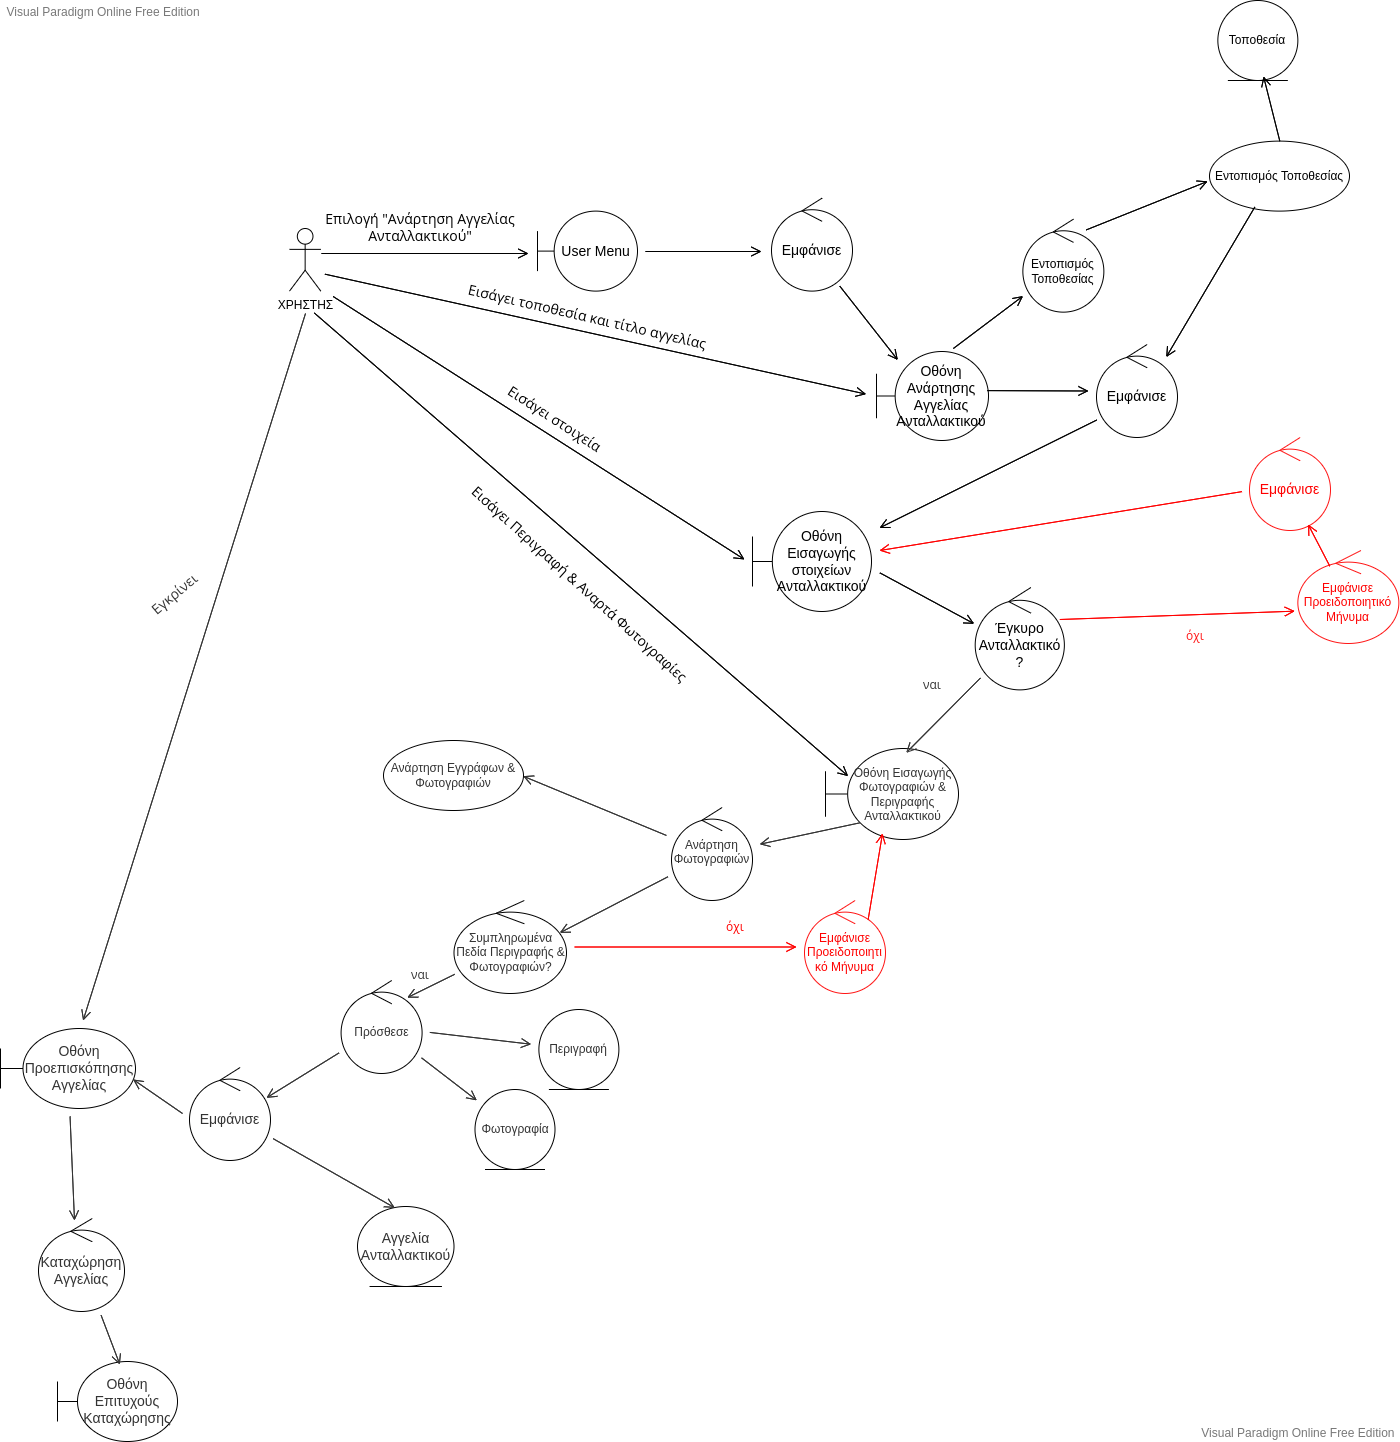
\includegraphics[scale=0.255]{img/rob_spare_part_listing.png}
		\caption{\en Robustness Diagram : "\gr Ανάρτηση Αγγελίας Πώλησης Ανταλλακτικού\en"\gr}
	\end{figure}
	
	\newpage
	\centering
	
	\paragraph{\en Use Case 12: \gr Έλεγχος Αναφοράς} 
	
	\begin{enumerate}
		\item Ο υπάλληλος της Ασφαλιστικής εταιρείας επιλέγει \en"\gr Έλεγχος Αναφοράς\en" \gr στο αρχικό μενού
		\item Το σύστημα εμφανίζει την οθόνη Καταχωρημένων Αναφορών, η οποία περιέχει την λίστα με τις αναφορές, τον κωδικό τους και την κατάστασή τους (\en"\gr σε εκκρεμότητα \en" \gr ή \en"\gr ελεγμένη\en"\gr)
		\item Ο υπάλληλος επιλέγει ή εισάγει τον κωδικό της αναφοράς που επιθυμεί να ελέγξει 
		\item Το σύστημα ελέγχει την εγκυρότητα του κωδικού αναφοράς και ανακτά την αναφορά αγγελίας
		\item Το σύστημα μεταφέρει τον χρήστη στην οθόνη Λεπτομέρειες Αναφοράς, εμφανίζοντας τον δημιουργό την αναφοράς, την ημερομηνία αλλά και την αιτία δημιουργίας της, καθώς και την αγγελία που αποτελεί αντικείμενο της αναφοράς, ενώ δίνει στον χρήστη την επιλογή να διαγράψει ή όχι την αγγελία
		\item Ο υπάλληλος της εταιρείας, εξετάζει την αναφορά και επιλέγει ενέργεια (διαγραφή ή όχι)
		\item Το σύστημα ελέγχει αν επιλέχθηκε διαγραφή της αγγελίας και μεταφέρει τον χρήστη στην οθόνη Διαγραφή Αγγελίας \footnote[2]{Θεωρούμε πως στην πλειοψηφία των περιπτώσεων, ο υπάλληλος θα προχωρήσει σε διαγραφή της αγγελίας. Δηλαδή, πως συνήθως, οι αναφορές είναι βάσιμες}
		\item Ο υπάλληλος συμπληρώνει την φόρμα, με την αιτία διαγραφής της αγγελίας, και προχωρά στην υποβολή της
		\item Το σύστημα διαγράφει την Αγγελία, αποστέλλει \en email \gr στον δημιουργό της αγγελίας, με ένα αντίγραφο της φόρμας Διαγραφής Αγγελίας που δημιούργησε ο υπάλληλος της εταιρείας. Τέλος, σημειώνει την αναφορά ως \textit{Ελεγμένη} και επιστρέφει τον υπάλληλο στο αρχικό μενού
	\end{enumerate}
	
	\paragraph{Εναλλακτική Ροή 1}
	\begin{enumerate}
		\item Ο υπάλληλος της ασφαλιστικής εταιρείας εισάγει κωδικό αναφοράς που δεν αντιστοιχεί σε κάποια καταχωρημένη αναφορά
		\item Το σύστημα εμφανίζει προειδοποιητικό μήνυμα και τον μεταφέρει στην οθόνη \textit{Καταχωρημένων Αναφορών}, προτρέποντάς τον να εισάγει ξανά τον κωδικό ή να επιλέξει μια αναφορά και η Περίπτωση Χρήσης συνεχίζει από το βήμα 3 της βασικής ροής
	\end{enumerate}	
	
	\paragraph{Εναλλακτική Ροή 2}
	\begin{enumerate}
		\item Ο υπάλληλος της ασφαλιστικής εταιρείας κρίνει πως η αγγελία δεν παραβιάζει κάποιον όρο της πλατφόρμας και δεν χρειάζεται να διαγραφεί
		\item Το σύστημα σημειώνει την αναφορά ως \textit{Ελεγμένη}	και επιστρέφει τον χρήστη στο αρχικό μενού
	\end{enumerate}
	
	\begin{figure}[htbp!]
		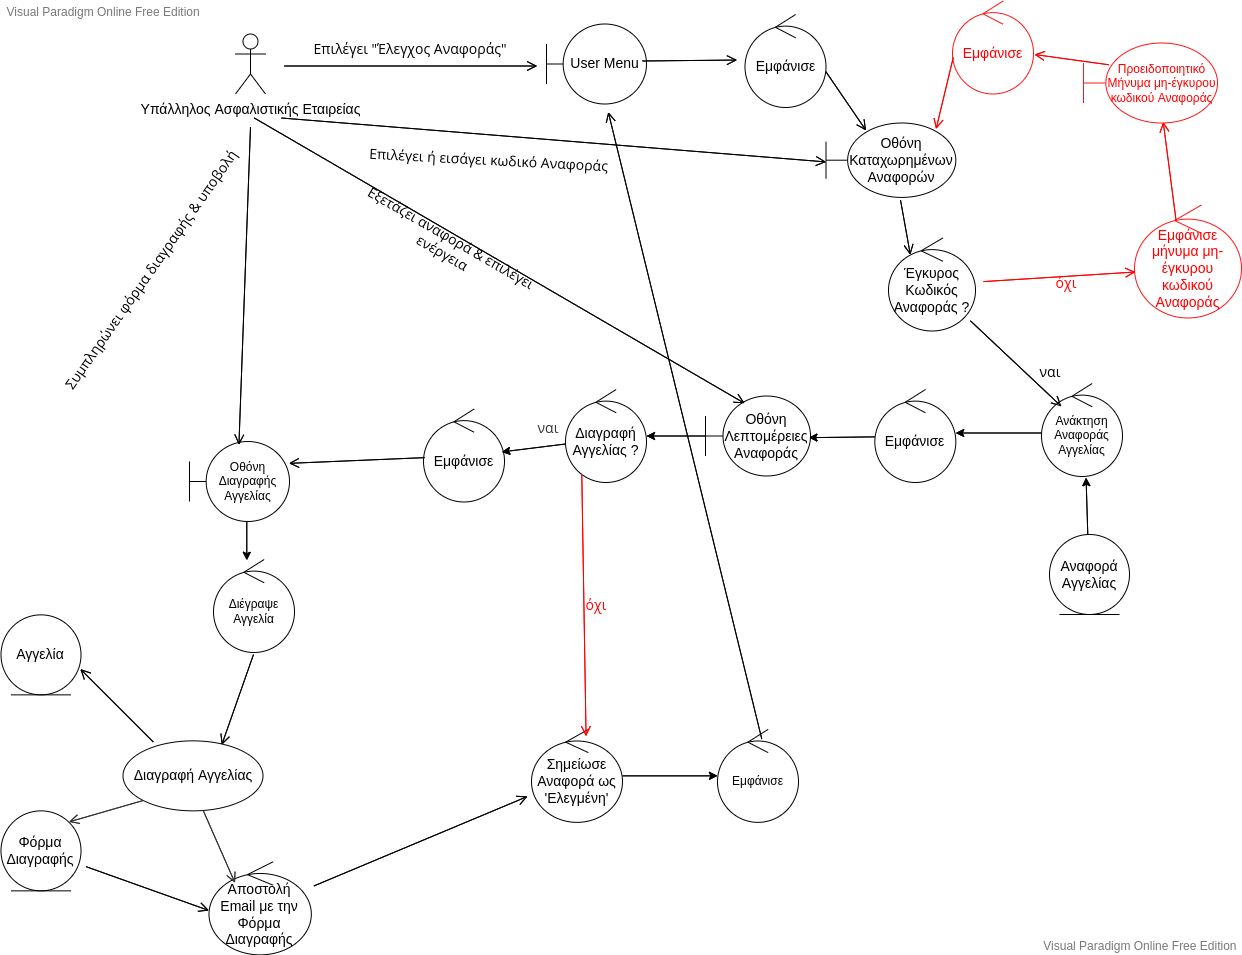
\includegraphics[scale=0.4]{img/rob_check_report.png}
		\caption{\en Robustness Diagram : "\gr Έλεγχος Αναφοράς\en"\gr}
	\end{figure}
	
	\newpage
	\centering
	
	\paragraph{\en Use Case 13: \gr Αγορά Ασφαλιστικού Πακέτου}
	\begin{enumerate}
		\item Ο χρήστης επιλέγει \en"\gr Αγορά Ασφαλιστικού Πακέτου\en" \gr στο αρχικό μενού
		\item Το σύστημα εμφανίζει την οθόνη Εισαγωγής Κωδικού Συναλλαγής
		\item Ο χρήστης εισάγει τον κωδικό της συναλλαγής, για το όχημα της οποίας επιθυμεί να αγοράσει ασφαλιστική κάλυψη
		\item Το σύστημα ελέγχει την εγκυρότητα του κωδικού συναλλαγής, και μεταφέρει τον χρήστη στην οθόνη Επιλογής Ασφαλιστικού Πακέτου, στην οποία εμφανίζονται τα στοιχεία της αγοράς του οχήματος. Το σύστημα προτρέπει τον χρήστη να επιλέξει το ασφαλιστικό πακέτο που επιθυμεί και να εισάγει το ποσό των πόντων που επιθυμεί να εξαργυρώσει, με σκοπό την εξασφάλιση έκπτωσης στα ασφάλιστρα \footnote[3]{Σε περίπτωση που ο χρήστης δεν επιθυμεί να εξαργυρώσει πόντους, μπορεί να εισάγει την τιμή \textbf{μηδέν} ως ποσό πόντων προς εξαργύρωση}
		\item Ο χρήστης επιλέγει ασφαλιστικό πακέτο και εισάγει το επιθυμητό ποσό πόντων προς εξαργύρωση
		\item Το σύστημα ανακτά το συνολικό ποσό πόντων του χρήστη και	ελέγχει αν διαθέτει το ποσό των πόντων που εισήχθησαν
		\item Το σύστημα εξαργυρώνει τους πόντους, υπολογίζει την τιμή των ασφαλίστρων και εμφανίζει την οθόνη Τιμή Ασφαλίστρων, όπου περιέχεται η τελική τιμή 
		\item Ο χρήστης αποδέχεται τα ασφάλιστρα
		\item Το σύστημα μεταφέρει τον χρήστη στο μενού πληρωμών. Μετά την επιτυχή πληρωμή, γίνεται καταχώρηση της συναλλαγής στο \en \textit{TransactionLog} \gr και δημιουργία του Ασφαλιστικού Πακέτου (Οντότητα \en \textit{InsurancePlan}\gr)
		\item Το σύστημα προσθέτει στο Ασφαλιστικό Συμβόλαιο τα απαραίτητα στοιχεία, στέλνει \en email \gr στον χρήστη με την απόδειξη της πληρωμής και τα στοιχεία του συμβολαίου. Τέλος, εμφανίζει οθόνη επιτυχούς αγοράς	
	\end{enumerate}
	
	\paragraph{Εναλλακτική Ροή 1 }
	
	\begin{enumerate}
		\item Ο χρήστης εισάγει κωδικό μη-καταγεγραμμένης συναλλαγής
		\item Το σύστημα εμφανίζει μήνυμα σφάλματος και επιστρέφει τον χρήστη στην  οθόνη \textit{Εισαγωγή Κωδικού Συναλλαγής}, προτρέποντάς τον να εισάγει έγκυρο κωδικό συναλλαγής
		\item Ο χρήστης επανεισάγει τον κωδικό και η Περίπτωση Χρήσης συνεχίζει από το βήμα 4 της βασικής ροής
	\end{enumerate}
	
	\paragraph{Εναλλακτική Ροή 2}
	\begin{enumerate}
		\item Ο χρήστης εισάγει παραπάνω πόντους από όσους έχει στην κατοχή του
		\item Το σύστημα εμφανίζει μήνυμα σφάλματος ενημερώνοντας τον χρήστη πως δεν διαθέτει το συγκεκριμένο πόσο πόντων.
		\item Το σύστημα επιστρέφει τον χρήστη στην οθόνη \textit{Επιλογής Ασφαλιστικού Πακέτου} και η Περίπτωση Χρήσης, συνεχίζει από το βήμα 5 της Βασικής Ροής
	\end{enumerate}
	
	\begin{figure}[htbp!]
		\includegraphics[scale=0.39]{img/rob\_purchase\_insurance\_plan.png}
		\caption{\en Robustness Diagram : "\gr Αγορά Ασφαλιστικού Πακέτου\en"\gr}
	\end{figure}
	
	\newpage
	\centering
	
	\paragraph{\en Use Case 14: \gr Μεταφορά Οχήματος}  
	\begin{enumerate}
		\item Ο χρήστης επιλέγει \en"\gr Μεταφορά Οχήματος\en" \gr στο αρχικό μενού
		\item Το σύστημα εμφανίζει την οθόνη Εισαγωγής Κωδικού Συναλλαγής και προτρέπει τον χρήστη να εισάγει τον κωδικό συναλλαγής
		\item Ο χρήστης εισάγει τον κωδικό που του είχε σταλεί μετά την ολοκλήρωση της αγοράς του οχήματος
		\item Το σύστημα αφού ελέγξει την εγκυρότητα του κωδικού συναλλαγής, εμφανίζει την οθόνη \en"\gr Τοποθεσία Παράδοσης Οχήματος\en" \gr, ώστε να εισάγει ο χρήστης το επιθυμητό σημείο παράδοσης
		\item Ο χρήστης εισάγει την τοποθεσία που επιθυμεί
		\item Το σύστημα εντοπίζει τον χρήστη. Έπειτα, εμφανίζει την οθόνη Επιλογής Υπηρεσίας Μεταφοράς, προτρέποντας τον χρήστη να επιλέξει την υπηρεσία μεταφοράς που επιθυμεί (\en express \gr παράδοση ή κανονική)		
		\item Ο χρήστης επιλέγει την υπηρεσία της αρεσκείας του
		\item Το σύστημα μεταφέρει τον χρήστη στην οθόνη \en"\gr Στοιχεία Μεταφοράς\en"\gr, εμφανίζοντας τα έξοδα της μεταφοράς, τα στοιχεία του μεταφορέα, το σημείο παράδοσης, τα στοιχεία του οχήματος καθώς και τον εκτιμώμενο χρόνο παράδοσης 
		\item Ο χρήστης επιβεβαιώνει την ορθότητα των στοιχείων 
		\item Το σύστημα αναζητά Μεταφορέα, δημιουργεί την Μεταφορά και προσθέτει σε αυτή τις απαραίτητες πληροφορίες. Έπειτα, μεταφέρει τον χρήστη στην οθόνη του συστήματος πληρωμών.
		\item Το σύστημα καταγράφει την συναλλαγή στο \en \textit{TransactionLog} \gr	και αποστέλλει \en email \gr στον Μεταφορέα αλλά και στον χρήστη με την απόδειξη της συναλλαγής. Τέλος, εμφανίζει μήνυμα επιτυχούς προγραμματισμού μεταφοράς
	\end{enumerate}
	
	\paragraph{Εναλλακτική Ροή}
	\begin{enumerate}
		\item Ο χρήστης εισάγει κωδικό μη-καταγεγραμμένης συναλλαγής
		\item Το σύστημα εμφανίζει μήνυμα μη-έγκυρου κωδικού συναλλαγής και επιστρέφει τον χρήστη στην οθόνη \textit{Εισαγωγή Κωδικού Συναλλαγής} 
		\item Ο χρήστης επανεισάγει τον κωδικό και η Περίπτωση Χρήσης συνεχίζει από το βήμα 3 της βασικής ροής
	\end{enumerate}
	
	\begin{figure}[htbp!]
		\includegraphics[scale=0.31]{img/rob\_car\_transport.png}
		\caption{\en Robustness Diagram : "\gr Μεταφορά Οχήματος\en"\gr}
	\end{figure}
	
	
	
	
	
	
	
	
	
	
\end{document}




